% Compile with XeLaTeX:  latexmk -xelatex Eval3_Presentation.tex   (font: Poppins, falls back if missing)
\documentclass[aspectratio=169,12pt]{beamer}
\usepackage{fontspec}
\IfFontExistsTF{Poppins}{\setsansfont{Poppins}[UprightFont=*-Regular,BoldFont=*-Bold,ItalicFont=*-Italic,BoldItalicFont=*-BoldItalic]}{}
\renewcommand{\familydefault}{\sfdefault}
\usepackage{tikz,booktabs,graphicx,array}
\usetikzlibrary{shapes,arrows.meta,positioning,calc,shadows}
\usepackage[most]{tcolorbox}
\definecolor{navy}{HTML}{0F1B3D}\definecolor{ink}{HTML}{1E2B4D}
\definecolor{accent}{HTML}{FF6B35}\definecolor{teal}{HTML}{14B8A6}
\definecolor{bg}{HTML}{F3F6FC}\definecolor{sky}{HTML}{4F6BFF}
\setbeamercolor{background canvas}{bg=bg}
\setbeamercolor{normal text}{fg=ink}
\setbeamertemplate{navigation symbols}{}
\setbeamersize{text margin left=13mm,text margin right=13mm}
\setbeamertemplate{itemize item}{\color{accent}$\blacksquare$}
\setbeamerfont{itemize/enumerate body}{size=\Large}
\hyphenpenalty=10000\exhyphenpenalty=10000\tolerance=2000\emergencystretch=3em
\AtBeginDocument{\raggedright}
\setbeamertemplate{background}{\begin{tikzpicture}[remember picture,overlay]
 \fill[sky!7](current page.south east)++(-6mm,-4mm) circle (30mm);
 \fill[accent!10](current page.south east)++(-40mm,-10mm) circle (12mm);
\end{tikzpicture}}
% header band
\setbeamertemplate{frametitle}{%
 \begin{tikzpicture}[remember picture,overlay]
  \shade[left color=navy,right color=ink!70!sky](current page.north west) rectangle ([yshift=-21mm]current page.north east);
  \fill[accent](current page.north west)++(0,-21mm) rectangle ++(38mm,-1.4mm);
  \fill[white,opacity=.06]([xshift=-14mm,yshift=2mm]current page.north east) circle (17mm);
  \node[anchor=west,text width=138mm,align=left,inner sep=0] at ([xshift=13mm,yshift=-10.5mm]current page.north west)
   {{\fontsize{8}{9}\selectfont\color{accent}\bfseries\MakeUppercase{\insertsection}\par}\vskip0.5mm
    {\fontsize{19}{21}\selectfont\color{white}\bfseries\insertframetitle\par}};
 \end{tikzpicture}\vskip6mm}
\setbeamertemplate{footline}{\leavevmode\hbox to\paperwidth{\hspace{13mm}{\fontsize{7}{8}\selectfont\color{navy!55}\bfseries INFRA-CVE\ \ |\ \ B.Tech Project Evaluation 3}\hfill
 \tikz[baseline=(n.base)]\node[fill=accent,text=white,rounded corners=2pt,inner xsep=2.2mm,inner ysep=0.8mm,font=\fontsize{7}{8}\selectfont\bfseries](n){\insertframenumber};\hspace{9mm}}\vskip3mm}
% ---------- components ----------
\newlength{\ch}\setlength{\ch}{47mm}
\tcbset{base/.style={enhanced,colback=white,colframe=white,boxrule=0pt,arc=3mm,drop fuzzy shadow=navy!35,halign=flush left}}
\newtcolorbox{tc}[3][]{base,width=0.94\linewidth,height=\ch,borderline north={1.6mm}{0pt}{accent},left=4mm,right=3mm,top=3mm,bottom=2mm,
 before upper={{\large\bfseries\color{navy}#3}\par\vskip1.2mm},
 overlay={\node[anchor=north east,font=\fontsize{24}{24}\selectfont\bfseries,text=navy!12] at ([xshift=-3mm,yshift=-3mm]frame.north east){#2};},#1}
\newtcolorbox{tcteal}[3][]{base,width=0.94\linewidth,height=\ch,borderline north={1.6mm}{0pt}{teal},left=4mm,right=3mm,top=3mm,bottom=2mm,
 before upper={{\large\bfseries\color{navy}#3}\par\vskip1.2mm},
 overlay={\node[anchor=north east,font=\fontsize{24}{24}\selectfont\bfseries,text=navy!12] at ([xshift=-3mm,yshift=-3mm]frame.north east){#2};},#1}
\newtcolorbox{wc}[1][]{base,borderline west={1.6mm}{0pt}{accent},left=5mm,right=4mm,top=3mm,bottom=3mm,#1}
\newtcolorbox{stmt}[1][]{enhanced,colback=navy,colframe=navy,coltext=white,boxrule=0pt,arc=3mm,drop fuzzy shadow=navy!40,halign=flush left,
 height={40mm},height plus=30mm,valign=center,left=7mm,right=6mm,fontupper=\fontsize{16}{23}\selectfont,
 overlay={\fill[accent,rounded corners=1pt]([xshift=2.5mm,yshift=-6mm]frame.north west) rectangle ([xshift=4mm,yshift=6mm]frame.south west);
          \fill[white,opacity=.05]([xshift=-6mm,yshift=2mm]frame.north east) circle (14mm);},#1}
\newtcolorbox{row}[1][]{base,height=10mm,fontupper=\small,valign=center,left=3mm,right=2mm,top=0mm,bottom=0mm,borderline west={1.4mm}{0pt}{accent},#1}
\newcommand{\ph}[1]{\textcolor{accent}{\textbf{[#1]}}}
\newcommand{\badge}[1]{\tikz[baseline=(n.base)]\node[circle,fill=accent,text=white,inner sep=0pt,minimum size=7mm,font=\small\bfseries](n){#1};}
\newcommand{\bignum}[2]{{\fontsize{16}{18}\selectfont\bfseries\color{accent}#1}\ {\footnotesize\color{ink!80}#2}}
\newcommand{\darkbg}{\begin{tikzpicture}[remember picture,overlay]
 \shade[left color=navy,right color=ink!80!sky](current page.south west) rectangle (current page.north east);
 \fill[accent,opacity=.92](current page.south east)++(-4mm,-8mm) circle (32mm);
 \fill[sky,opacity=.4](current page.north east)++(-20mm,4mm) circle (24mm);
 \fill[teal,opacity=.55](current page.south west)++(62mm,-4mm) circle (10mm);
\end{tikzpicture}}
\newcommand{\pill}[1]{\tikz[baseline=(n.base)]\node[draw=white,text=white,rounded corners=3mm,inner xsep=3mm,inner ysep=1.4mm,font=\footnotesize\bfseries,line width=.6pt](n){#1};}
% snake flow: 6 labels + optional store
\newcommand{\snake}[7]{\begin{center}\begin{tikzpicture}[
 n/.style={fill=navy,text=white,rounded corners=3pt,minimum width=38mm,minimum height=14mm,align=center,font=\bfseries\small,drop shadow={shadow xshift=.4mm,shadow yshift=-.4mm,opacity=.25}},
 a/.style={-{Stealth[length=2.6mm]},very thick,accent}]
 \node[n,fill=teal](a1)at(0,0){#1};\node[n](a2)at(47.5mm,0){#2};\node[n](a3)at(95mm,0){#3};
 \node[n](a4)at(95mm,-21mm){#4};\node[n](a5)at(47.5mm,-21mm){#5};\node[n,fill=accent](a6)at(0,-21mm){#6};
 \draw[a](a1)--(a2);\draw[a](a2)--(a3);\draw[a](a3)--(a4);\draw[a](a4)--(a5);\draw[a](a5)--(a6);
 \if\relax\detokenize{#7}\relax\else
 \node[n,fill=sky,minimum width=133mm,minimum height=10mm](st)at(47.5mm,-39mm){#7};
 \draw[sky,very thick,dashed,-{Stealth}](a5.south)--(st.north);\fi
\end{tikzpicture}\end{center}}
% terminal window
\newcommand{\term}[2]{\begin{tcolorbox}[enhanced,colback=black,colframe=black,boxrule=0pt,arc=2.5mm,boxsep=0pt,left=0pt,right=0pt,top=0pt,bottom=0pt,
 drop fuzzy shadow=navy!50,toptitle=1.3mm,bottomtitle=1.3mm,colbacktitle=ink,coltitle=white,fonttitle=\fontsize{7.5}{9}\selectfont\bfseries,
 title={{\color{red!80}$\bullet$}{\color{yellow!90!orange}$\bullet$}{\color{green!70!black}$\bullet$}\ \ #1}]
 \includegraphics[width=\linewidth]{#2}\end{tcolorbox}}
\newcommand{\shotframe}[4]{\begin{frame}{#1}\vskip-1mm
 \term{#2}{#3}\vskip2.5mm\begin{wc}[halign=center]#4\end{wc}\end{frame}}
\newcommand{\shotimg}[1]{\tcbox[enhanced,colback=white,colframe=white,boxrule=0pt,arc=2mm,boxsep=0pt,left=0pt,right=0pt,top=0pt,bottom=0pt,drop fuzzy shadow=black!60]{\includegraphics[height=0.88\paperheight]{#1}}}

\title{INFRA-CVE}
\begin{document}

\begin{frame}[plain]\darkbg\centering\vfill\shotimg{img/front.png}\vfill\end{frame}
\begin{frame}[plain]\darkbg\centering\vfill\shotimg{img/approval.png}\vfill\end{frame}

\begin{frame}[plain]\darkbg\vfill\color{white}
{\color{accent}\bfseries\fontsize{10}{12}\selectfont B.TECH PROJECT EVALUATION 3\ \ \textbullet\ \ RUBRIC \#R3}\\[2.5mm]
{\fontsize{50}{54}\selectfont\bfseries INFRA-CVE}\\[2mm]
{\fontsize{15}{20}\selectfont\bfseries A Provenance-Grounded, Confidence-Tiered\\Automatic CVE Checker for Entire Infrastructure}\\[3.5mm]
\pill{Provenance-grounded}\ \pill{Confidence-tiered}\ \pill{Read-only}\\[4mm]
{\small Initial Implementation and Synchronization\\[0.5mm]
Department of Computer Science \& Engineering, Sharda School of Engineering and Technology\ \ \textbullet\ \ October 2026}
\vfill\end{frame}

\begin{frame}{Table of Contents}
\normalsize
\begin{columns}[T,onlytextwidth]\column{.52\textwidth}
\begin{tabular}{@{}c@{\hskip3mm}l@{}}
\badge1&Introduction and Overview\\[2.4mm]
\badge2&Problem and Objectives\\[2.4mm]
\badge3&Scope and Specifications\\[2.4mm]
\badge4&System Requirements\\[2.4mm]
\badge5&SDLC Model Selection\\[2.4mm]
\badge6&Tools and Technologies\\[2.4mm]
\badge7&System Design and Architecture
\end{tabular}
\column{.48\textwidth}
\begin{tabular}{@{}c@{\hskip3mm}l@{}}
\badge8&Appropriateness of Design\\[2.4mm]
\badge9&Synchronization with Design\\[2.4mm]
\badge{10}&Implementation and Demos\\[2.4mm]
\badge{11}&Results and Discussion\\[2.4mm]
\badge{12}&Conclusion and Future Work\\[2.4mm]
\badge{13}&References and Q\&A
\end{tabular}\end{columns}
\end{frame}

\begin{frame}{Project, Team and Guide}
\begin{stmt}[height={14mm},height plus=30mm,fontupper=\normalsize]\textbf{INFRA-CVE} checks entire infrastructure against known CVEs with provenance and honest confidence.\end{stmt}
\vskip2mm\setlength{\ch}{20mm}
\begin{columns}[T,onlytextwidth]
\column{.34\textwidth}\begin{tc}{1}{\normalsize Itesh Jung Shahi}\small ID 2023837775\end{tc}
\column{.33\textwidth}\begin{tc}{2}{\normalsize Amit Kumar}\small ID 2023345474\end{tc}
\column{.33\textwidth}\begin{tc}{3}{\normalsize\ph{Student 3}}\small ID \ph{insert}\end{tc}
\end{columns}\vskip1.5mm
\begin{wc}[borderline west={1.6mm}{0pt}{teal}]\small\textbf{Mentor / Guide:} Dr.\ Deepthi P S, Associate Professor, CSE, Sharda School of Engineering and Technology\end{wc}
\end{frame}

\section{Introduction and Overview}
\begin{frame}{Introduction}
\begin{columns}[c,onlytextwidth]
\column{.4\textwidth}\centering{\fontsize{72}{74}\selectfont\bfseries\color{accent}92\%}\\[1mm]{\bfseries false positives in existing\\infrastructure CVE tooling,\\even on verified SBOMs}
\column{.6\textwidth}\begin{stmt}[height={46mm},height plus=30mm,fontupper=\fontsize{14}{20}\selectfont]No prior work has measured the \textbf{composed discovery-to-confidence pipeline} against ground truth.\end{stmt}
\end{columns}
\end{frame}

\begin{frame}{Project Overview}
\setlength{\ch}{27mm}
\begin{stmt}[height={19mm},height plus=30mm,fontupper=\fontsize{13}{18}\selectfont]INFRA-CVE reads installed software, checks trusted advisories, applies distro-aware logic, and reports \textbf{honest confidence tiers}.\end{stmt}\vskip2.5mm
\begin{columns}[T,onlytextwidth]
\column{.33\textwidth}\begin{tc}{01}{Read}\normalsize System package DB or manifest, normalised\end{tc}
\column{.33\textwidth}\begin{tcteal}{02}{Check}\normalsize OSV, Debian and Alpine advisories\end{tcteal}
\column{.33\textwidth}\begin{tc}{03}{Report}\normalsize Provenance stored, confidence-tiered\end{tc}
\end{columns}
\end{frame}

\section{Problem and Objectives}
\begin{frame}{Problem Statement}
\setlength{\ch}{50mm}
\begin{columns}[T,onlytextwidth]
\column{.5\textwidth}\begin{tc}{01}{Today}\normalsize Organisations run many systems, applications and packages. Most tools only match \textbf{package name + version} against a CVE list.\end{tc}
\column{.5\textwidth}\begin{tcteal}{02}{The consequence}\normalsize Huge false-alert counts: \textbf{backports} patch older versions without changing the upstream version.\end{tcteal}
\end{columns}
\end{frame}

\begin{frame}{Objectives}
\setlength{\ch}{25mm}
\begin{columns}[T,onlytextwidth]
\column{.5\textwidth}\begin{tc}{01}{Reduce false alerts}\normalsize Fewer wrong CVE findings\end{tc}\vskip2.5mm\begin{tc}{03}{Honest confidence}\normalsize Tiers, never overclaiming\end{tc}
\column{.5\textwidth}\begin{tcteal}{02}{Record evidence}\normalsize Clear proof for every finding\end{tcteal}\vskip2.5mm\begin{tcteal}{04}{Simple and safe}\normalsize Readable by non-technical users\end{tcteal}
\end{columns}
\end{frame}

\section{Scope and Specifications}
\begin{frame}{Scope of the Project}
\begin{stmt}[height={14mm},height plus=30mm,fontupper=\Large]\textbf{MVP scope}\end{stmt}\vskip2.5mm\setlength{\ch}{31mm}
\begin{columns}[T,onlytextwidth]
\column{.5\textwidth}\begin{tc}{A}{Inputs}\normalsize Linux host package DBs (dpkg/apk), manifests, banner probes\end{tc}
\column{.5\textwidth}\begin{tcteal}{B}{Analysis}\normalsize OSV lookup, distro-aware applicability, verification, scoring, reporting\end{tcteal}
\end{columns}
\end{frame}

\begin{frame}{Functional Specifications (CO4)}
\begin{stmt}[height={14mm},height plus=30mm,fontupper=\Large]Requirements \textbf{FR1--FR8} cover:\end{stmt}\vskip2.5mm\setlength{\ch}{31mm}
\begin{columns}[T,onlytextwidth]
\column{.5\textwidth}\begin{tc}{A}{Input and lookup}\normalsize Asset input, identity mapping, version normalisation, advisory lookup\end{tc}
\column{.5\textwidth}\begin{tcteal}{B}{Decide and report}\normalsize Distro-aware check, provenance storage, confidence tiers, simple report\end{tcteal}
\end{columns}
\end{frame}

\section{System Requirements}
\begin{frame}{Identified System Requirements}
\setlength{\ch}{50mm}
\begin{columns}[T,onlytextwidth]
\column{.5\textwidth}\begin{tc}{HW}{Hardware}\large Intel Core i3 or higher\\4 GB RAM min.\ (8 GB preferred)\\50 GB free disk space\end{tc}
\column{.5\textwidth}\begin{tcteal}{SW}{Software}\normalsize Linux / Windows, Python 3.10+, SQLite, requests, packaging, python-dateutil\\OSV.dev, Debian Security Tracker, Alpine secdb\end{tcteal}
\end{columns}
\end{frame}

\begin{frame}{Functional Requirements List}
\begin{columns}[T,onlytextwidth]
\column{.5\textwidth}
\begin{row}\textbf{\color{accent}FR1}\ \ Read-only input\end{row}\vskip0.8mm
\begin{row}\textbf{\color{accent}FR2}\ \ Map packages to PURL\end{row}\vskip0.8mm
\begin{row}\textbf{\color{accent}FR3}\ \ Normalise versions\end{row}\vskip0.8mm
\begin{row}\textbf{\color{accent}FR4}\ \ OSV + distro lookup\end{row}
\column{.5\textwidth}
\begin{row}\textbf{\color{accent}FR5}\ \ Prefer distro fix info\end{row}\vskip0.8mm
\begin{row}\textbf{\color{accent}FR6}\ \ Store provenance\end{row}\vskip0.8mm
\begin{row}\textbf{\color{accent}FR7}\ \ Confidence tiers\end{row}\vskip0.8mm
\begin{row}\textbf{\color{accent}FR8}\ \ Simple report with proof\end{row}
\end{columns}
\end{frame}

\begin{frame}{Non-Functional Requirements}
\setlength{\ch}{25mm}
\begin{columns}[T,onlytextwidth]
\column{.33\textwidth}\begin{tc}{1}{Safety}\normalsize Strictly read-only\end{tc}\vskip2.5mm\begin{tc}{4}{Reproducible}\normalsize Same input, same result\end{tc}
\column{.33\textwidth}\begin{tcteal}{2}{Clarity}\normalsize Easy for non-technical users\end{tcteal}\vskip2.5mm\begin{tcteal}{5}{Lightweight}\normalsize Runs on a normal laptop\end{tcteal}
\column{.33\textwidth}\begin{tc}{3}{Honesty}\normalsize Says ``unknown'' without proof\end{tc}\vskip2.5mm\begin{tc}{6}{Evidence-based}\normalsize Every CVE has stored evidence\end{tc}
\end{columns}
\end{frame}

\begin{frame}{Quantification and Completeness Analysis}
\begin{columns}[c,onlytextwidth]
\column{.4\textwidth}\centering{\fontsize{66}{68}\selectfont\bfseries\color{accent}92\%}\\[1mm]{\bfseries baseline false-positive rate}
\column{.6\textwidth}\begin{wc}[height={44mm},height plus=30mm,valign=center]\large Downstream scanners show this rate even with verified SBOMs. The MVP was quantified against \textbf{live scans} (banner, inventory, web app) to show honest behaviour.\end{wc}
\end{columns}
\end{frame}

\section{SDLC Model Selection}
\begin{frame}{Selection of SDLC Model (CO4)}
\begin{stmt}Selected model:\\[2mm]\textcolor{accent}{\bfseries[insert chosen model, e.g.\ Agile / Waterfall]}\end{stmt}
\end{frame}

\begin{frame}{Evaluation of Different SDLC Models}
\setlength{\ch}{36mm}
\begin{columns}[T,onlytextwidth]
\column{.5\textwidth}\begin{tc}{A}{Agile iteration}\large Rapid demos and incremental delivery\end{tc}
\column{.5\textwidth}\begin{tcteal}{W}{Waterfall gates}\large Phase gates suit safety-critical checks\end{tcteal}
\end{columns}\vskip2mm
\begin{wc}\normalsize Compared against: safety-critical advisory checking, rapid demo, academic timeline.\ \ph{add comparison table}\end{wc}
\end{frame}

\begin{frame}{Justification for Selected Model}
\setlength{\ch}{50mm}
\begin{columns}[T,onlytextwidth]
\column{.33\textwidth}\begin{tc}{01}{Safety}\large Read-only constraints\end{tc}
\column{.33\textwidth}\begin{tcteal}{02}{Speed}\large Rapid evaluation delivery\end{tcteal}
\column{.33\textwidth}\begin{tc}{03}{Deadlines}\large Academic timeline\end{tc}
\end{columns}
\end{frame}

\begin{frame}{Implementation Strategy}
\snake{Discovery}{Advisory\\ingest}{Applicability}{Verification}{Scoring}{Report}{}
\begin{wc}[halign=center]\normalsize Incrementally demoed on Debian 12 hosts and a web application (Juice Shop)\end{wc}
\end{frame}

\section{Tools and Technologies}
\begin{frame}{Use of Latest Design Tools (CO5)}
\begin{stmt}Current design and authoring tools were used for diagrams, reports and code, supporting the \textbf{design-to-implementation synchronisation} requirement.\end{stmt}
\end{frame}

\begin{frame}{Tools and Technologies Used}
\setlength{\ch}{50mm}
\begin{columns}[T,onlytextwidth]
\column{.5\textwidth}\begin{tc}{</>}{Code and quality}\large Python, pydantic, httpx, pytest, mypy, ruff, Docker\end{tc}
\column{.5\textwidth}\begin{tcteal}{DB}{Data and docs}\large OSV.dev, Debian Security Tracker, Alpine secdb, SQLite, Markdown, \LaTeX{}\end{tcteal}
\end{columns}
\end{frame}

\begin{frame}{Reason for Tool Selection}
\begin{stmt}\fontsize{24}{28}\selectfont\textbf{100\% free and open source}\\[3mm]\normalsize\color{white!85!navy}No paid software, API or license. Runs on a normal laptop.\end{stmt}
\end{frame}

\section{System Design and Architecture}
\begin{frame}{Advantages and Relevance (CO4)}
\setlength{\ch}{25mm}
\begin{columns}[T,onlytextwidth]
\column{.5\textwidth}\begin{tc}{1}{Provenance}\normalsize Grounded decisions\end{tc}\vskip2.5mm\begin{tc}{3}{Honest}\normalsize Confidence tiers\end{tc}
\column{.5\textwidth}\begin{tcteal}{2}{Distro-first}\normalsize Version logic\end{tcteal}\vskip2.5mm\begin{tcteal}{4}{Simple}\normalsize Reporting\end{tcteal}
\end{columns}
\end{frame}

\begin{frame}{System Architecture Diagram}
\snake{Discovery}{Ingest}{Applicability}{Verification}{Scoring}{Report}{SQLite provenance store}
\end{frame}

\begin{frame}{Data Flow / UML Diagram}
\begin{center}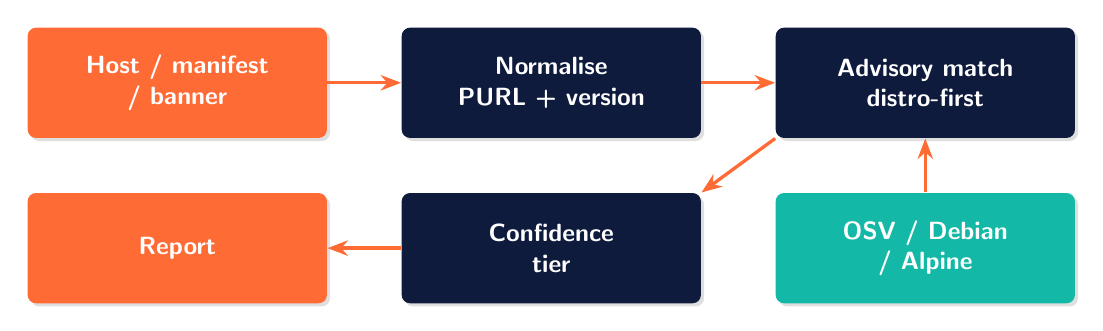
\begin{tikzpicture}[
 n/.style={fill=navy,text=white,rounded corners=3pt,minimum width=38mm,minimum height=14mm,align=center,font=\bfseries\small,drop shadow={shadow xshift=.4mm,shadow yshift=-.4mm,opacity=.25}},
 a/.style={-{Stealth[length=2.6mm]},very thick,accent}]
 \node[n,fill=accent](i)at(0,0){Host / manifest\\/ banner};\node[n](p)at(47.5mm,0){Normalise\\PURL + version};\node[n](m)at(95mm,0){Advisory match\\distro-first};
 \node[n,fill=teal](s)at(95mm,-21mm){OSV / Debian\\/ Alpine};\node[n](c)at(47.5mm,-21mm){Confidence\\tier};\node[n,fill=accent](r)at(0,-21mm){Report};
 \draw[a](i)--(p);\draw[a](p)--(m);\draw[a](s)--(m);\draw[a](m.south west)--(c.north east);\draw[a](c)--(r);
\end{tikzpicture}\end{center}
\end{frame}

\begin{frame}{Database Design}
\begin{stmt}[height={14mm},height plus=30mm,fontupper=\Large]\textbf{SQLite provenance store}\end{stmt}\vskip2.5mm\setlength{\ch}{31mm}
\begin{columns}[T,onlytextwidth]
\column{.5\textwidth}\begin{tc}{A}{Versions}\normalsize Raw version, normalised version, source and timestamp\end{tc}
\column{.5\textwidth}\begin{tcteal}{B}{Evidence}\normalsize Advisory source, reason, evidence link\end{tcteal}
\end{columns}
\end{frame}

\section{Appropriateness of Design}
\begin{frame}{Appropriateness of Design (CO4)}
\begin{stmt}The design maps directly to the requirements \textbf{without scope creep}.\end{stmt}
\end{frame}

\begin{frame}{Design Principles Applied}
\setlength{\ch}{25mm}
\begin{columns}[T,onlytextwidth]
\column{.5\textwidth}\begin{tc}{1}{Provenance-grounded}\normalsize Every decision has a source\end{tc}\vskip2.5mm\begin{tc}{3}{Confidence tiers}\normalsize Graded, never absolute\end{tc}
\column{.5\textwidth}\begin{tcteal}{2}{Distro-first}\normalsize Distro fix over upstream range\end{tcteal}\vskip2.5mm\begin{tcteal}{4}{Honest unknowns}\normalsize Unknown when proof is missing\end{tcteal}
\end{columns}
\end{frame}

\begin{frame}{Modularity and Scalability}
\begin{stmt}Modules are \textbf{small and single-purpose}, so new ecosystems and asset types can be added with little change.\end{stmt}
\end{frame}

\begin{frame}{Design Validation and Review}
\begin{stmt}The design was reviewed against the requirements and threats to validity \textbf{before implementation}.\end{stmt}
\end{frame}

\section{Synchronization with Design}
\begin{frame}{Synchronization with Design (CO4, CO5)}
\setlength{\ch}{50mm}
\begin{columns}[T,onlytextwidth]
\column{.5\textwidth}\begin{tc}{A}{Front half}\large Asset reader, identity resolver, version normaliser, advisory ingestor\end{tc}
\column{.5\textwidth}\begin{tcteal}{B}{Back half}\large Applicability engine, provenance store, confidence engine, report generator\end{tcteal}
\end{columns}
\end{frame}

\begin{frame}{Mapping Requirements to Components}
\begin{columns}[T,onlytextwidth]
\column{.5\textwidth}
\begin{row}\textbf{\color{accent}FR1}\ \ Asset reader\end{row}\vskip0.8mm
\begin{row}\textbf{\color{accent}FR2}\ \ Identity resolver\end{row}\vskip0.8mm
\begin{row}\textbf{\color{accent}FR3}\ \ Version normaliser\end{row}\vskip0.8mm
\begin{row}\textbf{\color{accent}FR4}\ \ Advisory ingestor\end{row}
\column{.5\textwidth}
\begin{row}\textbf{\color{accent}FR5}\ \ Applicability engine\end{row}\vskip0.8mm
\begin{row}\textbf{\color{accent}FR6}\ \ Provenance store\end{row}\vskip0.8mm
\begin{row}\textbf{\color{accent}FR7}\ \ Confidence engine\end{row}\vskip0.8mm
\begin{row}\textbf{\color{accent}FR8}\ \ Report generator\end{row}
\end{columns}
\end{frame}

\begin{frame}{Integration and Testing}
\begin{stmt}Integration and testing across \textbf{discovery, ingest, applicability, verification and report}.\end{stmt}
\end{frame}

\begin{frame}{Traceability Matrix}
\begin{stmt}Requirement $\rightarrow$ implementation $\rightarrow$ result\\[3mm]\fontsize{13}{16}\selectfont\ph{add requirement / module / test table}\end{stmt}
\end{frame}

\section{Implementation and Demos}
\begin{frame}{Implementation Overview}
\begin{stmt}[height={14mm},height plus=30mm,fontupper=\Large]MVP modules under \texttt{src/infravce/}\end{stmt}\vskip2.5mm\setlength{\ch}{31mm}
\begin{columns}[T,onlytextwidth]
\column{.5\textwidth}\begin{tc}{A}{Pipeline}\normalsize discovery, advisories, applicability, verification\end{tc}
\column{.5\textwidth}\begin{tcteal}{B}{Output}\normalsize reporting, prioritisation, CLI\end{tcteal}
\end{columns}
\end{frame}

\begin{frame}{Modules Developed}
\begin{columns}[T,onlytextwidth]
\column{.5\textwidth}
\begin{row}\textbf{\color{accent}discovery}\ \ \small reads inputs\end{row}\vskip0.8mm
\begin{row}\textbf{\color{accent}advisories}\ \ \small OSV, Debian, Alpine\end{row}\vskip0.8mm
\begin{row}\textbf{\color{accent}applicability}\ \ \small distro-aware\end{row}\vskip0.8mm
\begin{row}\textbf{\color{accent}verification}\ \ \small evidence checks\end{row}
\column{.5\textwidth}
\begin{row}\textbf{\color{accent}reporting}\ \ \small Markdown reports\end{row}\vskip0.8mm
\begin{row}\textbf{\color{accent}prioritisation}\ \ \small severity order\end{row}\vskip0.8mm
\begin{row}\textbf{\color{accent}CLI}\ \ \small \texttt{infravce.cli scan}\end{row}
\end{columns}
\end{frame}

\shotframe{Demo 1: Banner Scan}{infravce.cli scan --target 127.0.0.1 --ports 22,80}{img/banner_scan_crop.png}
{\bignum{2}{obs.}\ \ \textcolor{navy!30}{|}\ \ \bignum{386}{advisories}\ \ \textcolor{navy!30}{|}\ \ \bignum{58}{findings}\ \ \textcolor{navy!30}{|}\ \ \bignum{weak}{tier}}
\shotframe{Demo 2: Inventory Scan}{infravce.cli scan --inventory ... --fixed-only}{img/inventory_scan_crop.png}
{\bignum{88}{obs.}\ \ \textcolor{navy!30}{|}\ \ \bignum{155}{advisories}\ \ \textcolor{navy!30}{|}\ \ \bignum{58}{findings}\ \ \textcolor{navy!30}{|}\ \ \bignum{56}{strong}}
\shotframe{Demo 3: Juice Shop Web App Scan}{infravce.cli scan testing\_apps/juice-shop}{img/juice_shop_crop.png}
{\bignum{147}{obs.}\ \ \textcolor{navy!30}{|}\ \ \bignum{125}{advisories}\ \ \textcolor{navy!30}{|}\ \ \bignum{71}{findings}\ \ \textcolor{navy!30}{|}\ \ \bignum{critical}{top CVE}}

\begin{frame}{Key Features: Flow}
\snake{Banner / inventory / app}{Observations}{Advisory\\records}{Votes}{Findings\\+ tier}{Report}{}
\begin{wc}[halign=center]\normalsize Each scan writes observations, votes, findings, coverage and a report\end{wc}
\end{frame}

\section{Results and Discussion}
\begin{frame}{Results and Discussion}
\setlength{\ch}{50mm}
\begin{columns}[T,onlytextwidth]
\column{.33\textwidth}\begin{tc}{01}{Banner}{\fontsize{34}{36}\selectfont\bfseries\color{accent}58}\\\normalsize findings, all weak\end{tc}
\column{.33\textwidth}\begin{tcteal}{02}{Inventory}{\fontsize{34}{36}\selectfont\bfseries\color{accent}58}\\\normalsize 56 strongly inferred, 2 weak\end{tcteal}
\column{.33\textwidth}\begin{tc}{03}{Juice Shop}{\fontsize{34}{36}\selectfont\bfseries\color{accent}71}\\\normalsize top: CVE-2015-9235\end{tc}
\end{columns}
\end{frame}

\begin{frame}{Achieved Outcomes}
\setlength{\ch}{50mm}
\begin{columns}[T,onlytextwidth]
\column{.33\textwidth}\begin{tc}{01}{MVP}\large Delivered\end{tc}
\column{.33\textwidth}\begin{tcteal}{02}{Tests}\large Green\end{tcteal}
\column{.33\textwidth}\begin{tc}{03}{Demos}\large Live, validated\end{tc}
\end{columns}
\end{frame}

\begin{frame}{Comparison with Objectives}
\begin{stmt}Outcomes compared against the seven project objectives. Banner-only evidence is honestly tiered \emph{weak}; inventory scans reach \emph{strongly inferred}.\end{stmt}
\end{frame}

\section{Conclusion and Future Work}
\begin{frame}{Conclusion and Summary}
\begin{stmt}[height={26mm},height plus=30mm,fontupper=\fontsize{16}{22}\selectfont]INFRA-CVE demonstrates provenance-grounded, confidence-tiered CVE checking.\end{stmt}\vskip2.5mm
\begin{wc}\large Work done: discovery, ingest, matching, verification, reporting, tests and demos.\end{wc}
\end{frame}

\begin{frame}{Limitations}
\setlength{\ch}{50mm}
\begin{columns}[T,onlytextwidth]
\column{.33\textwidth}\begin{tc}{01}{Banner mapping}\large Live web-app banners\end{tc}
\column{.33\textwidth}\begin{tcteal}{02}{Coverage}\large Specific ecosystems only\end{tcteal}
\column{.33\textwidth}\begin{tc}{03}{Freshness}\large Advisory data age\end{tc}
\end{columns}
\end{frame}

\begin{frame}{Future Enhancements}
\setlength{\ch}{25mm}
\begin{columns}[T,onlytextwidth]
\column{.5\textwidth}\begin{tc}{1}{More ecosystems}\normalsize Beyond dpkg, apk, npm\end{tc}\vskip2.5mm\begin{tc}{3}{Container SBOMs}\normalsize Image scanning\end{tc}
\column{.5\textwidth}\begin{tcteal}{2}{CI/CD integration}\normalsize Gate builds\end{tcteal}\vskip2.5mm\begin{tcteal}{4}{Issue export}\normalsize Push to trackers\end{tcteal}
\end{columns}
\end{frame}

\section{References}
\begin{frame}{References}
\begin{wc}[height={48mm},height plus=30mm,valign=center]\Large OSV.dev\\Debian Security Tracker\\Alpine secdb\\arXiv:2511.20313\\Project documentation\end{wc}
\end{frame}

\begin{frame}{Tools, Frameworks and Papers}
\setlength{\ch}{50mm}
\begin{columns}[T,onlytextwidth]
\column{.5\textwidth}\begin{tc}{A}{Tools}\large Python, pydantic, httpx, pytest, mypy, ruff, Docker\end{tc}
\column{.5\textwidth}\begin{tcteal}{B}{Research}\large Grype / Trivy, SBOM studies\end{tcteal}
\end{columns}
\end{frame}

\begin{frame}[plain]\darkbg\centering\vfill\color{white}
{\fontsize{54}{58}\selectfont\bfseries Q\&A}\\[3mm]{\color{accent}\rule{24mm}{1.4mm}}\\[3mm]{\Huge Thank you}\vfill\end{frame}
\end{document}
